% Editable vector version of rotating-calipers2.png.
% Regenerate from this directory:
% latex -interaction=nonstopmode -halt-on-error rotating-calipers-2.tex
% dvisvgm --no-fonts --exact --bbox=papersize --output=rotating-calipers-2.svg rotating-calipers-2.dvi
\documentclass[tikz,border=0pt]{standalone}
\usepackage[T1]{fontenc}
\usepackage{newtxtext,newtxmath}
\usetikzlibrary{calc,decorations.pathreplacing}
\definecolor{supportred}{RGB}{237,28,36}
\definecolor{projectionblue}{RGB}{0,174,239}
\definecolor{projectionyellow}{RGB}{244,218,0}
\definecolor{trianglepurple}{RGB}{163,73,164}
\begin{document}
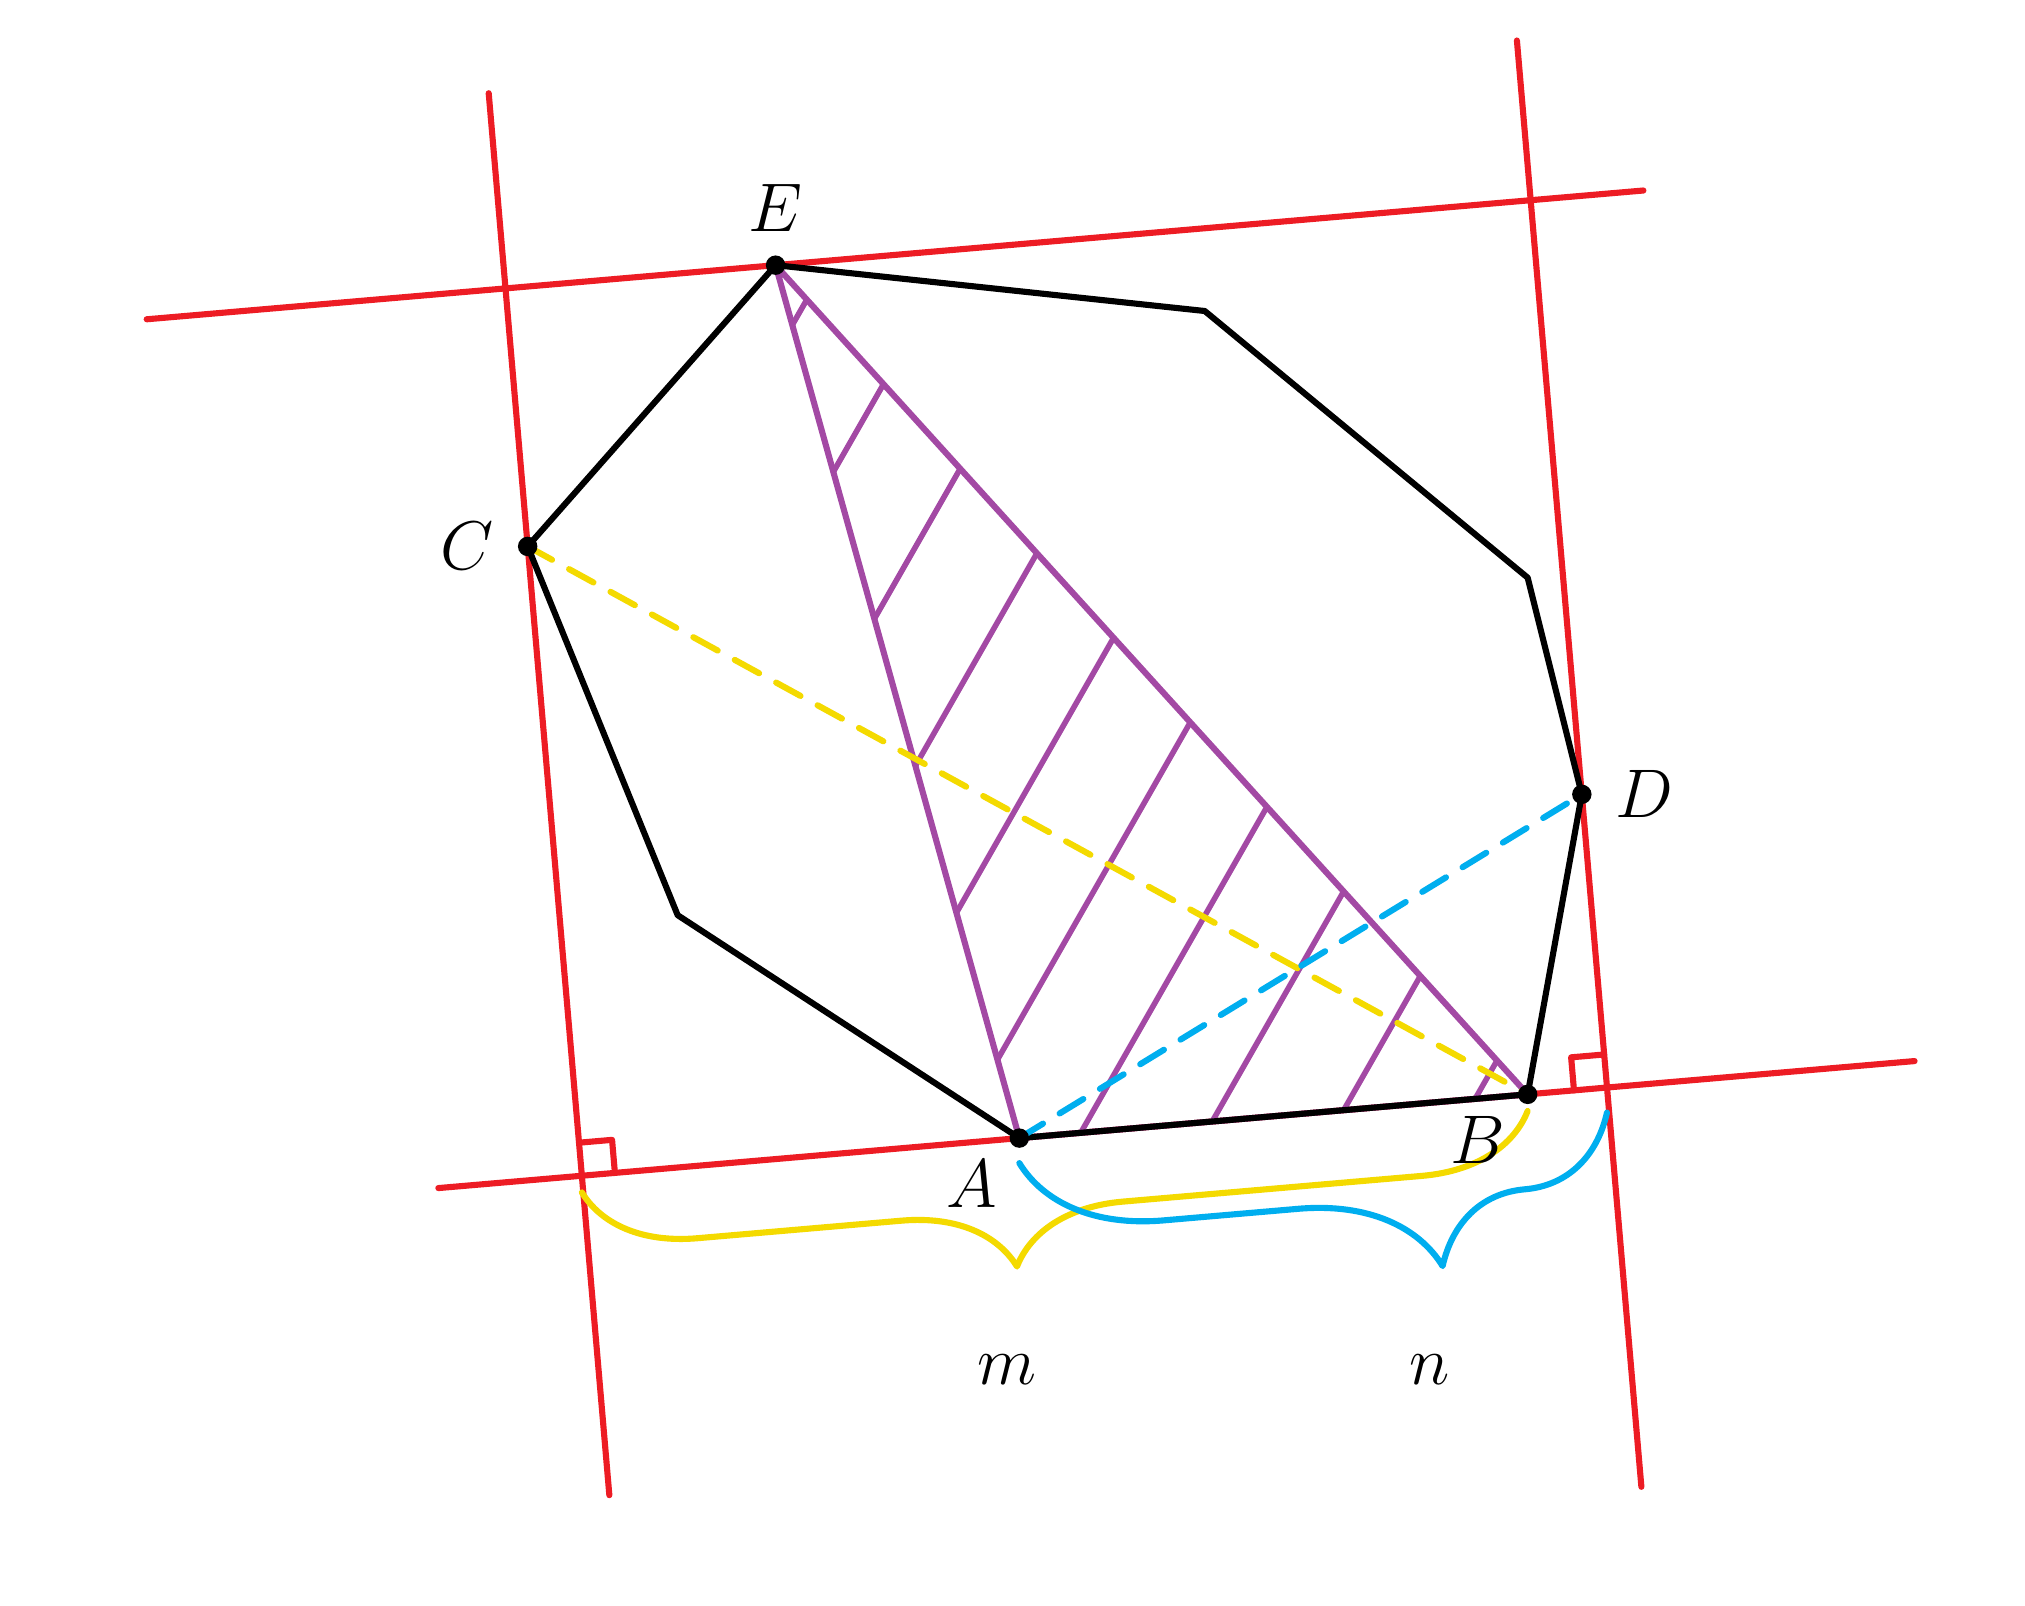
\begin{tikzpicture}[x=0.75bp,y=-0.75bp,
  line cap=round,line join=round,line width=2.2bp,
  every node/.style={inner sep=3bp,font=\fontsize{28bp}{32bp}\selectfont}]
  \path[use as bounding box] (0,0) rectangle (945,744);
  \clip (0,0) rectangle (945,744);
  \fill[white] (0,0) rectangle (945,744);
  \coordinate (A) at (476,533);
  \coordinate (B) at (720,512);
  \coordinate (C) at (240,249);
  \coordinate (D) at (746,368);
  \coordinate (E) at (359,114);
  \coordinate (edge) at ($(B)-(A)$);
  \coordinate (normal) at (-21,-244);

  % Orthogonal projections onto AB determine the left/right supports.
  \coordinate (L) at ($(A)!(C)!(B)$);
  \coordinate (R) at ($(A)!(D)!(B)$);
  \coordinate (F) at ($(A)!(E)!(B)$);
  \coordinate (height) at ($(E)-(F)$);
  \coordinate (TL) at ($(L)+(height)$);
  \coordinate (TR) at ($(R)+(height)$);
  \draw[supportred] ($(L)!-0.36!(TL)$) -- ($(L)!1.22!(TL)$);
  \draw[supportred] ($(R)!-0.45!(TR)$) -- ($(R)!1.18!(TR)$);
  \draw[supportred] ($(TL)!-0.35!(TR)$) -- ($(TL)!1.11!(TR)$);
  \draw[supportred] ($(L)!-0.14!(R)$) -- ($(L)!1.3!(R)$);
  \draw[supportred] ($(L)+0.065*(edge)$)
    -- ($(L)+0.065*(edge)+0.065*(normal)$) -- ($(L)+0.065*(normal)$);
  \draw[supportred] ($(R)-0.065*(edge)$)
    -- ($(R)-0.065*(edge)+0.065*(normal)$) -- ($(R)+0.065*(normal)$);

  % Twice the purple area is S = |AB| times the rectangle's height.
  \begin{scope}
    \clip (A) -- (E) -- (B) -- cycle;
    \foreach \offset in {-100,-40,...,920} {
      \draw[trianglepurple,line width=2bp]
        (\offset,750) -- (\offset+400,50);
    }
  \end{scope}
  \draw[trianglepurple] (A) -- (E) -- (B) -- cycle;
  \draw (A) -- (B) -- (D) -- (720,264) -- (565,136) -- (E)
    -- (C) -- (312,426) -- cycle;
  \draw[projectionyellow,dash pattern=on 10bp off 7bp] (C) -- (B);
  \draw[projectionblue,dash pattern=on 10bp off 7bp] (A) -- (D);

  % m = |LB| and n = |AR|, hence the rectangle's width is m + n - |AB|.
  \draw[projectionyellow,decorate,
    decoration={brace,mirror,amplitude=40bp,aspect=0.45}]
    ($(L)+(0,8)$) -- ($(B)+(0,8)$);
  \draw[projectionblue,decorate,
    decoration={brace,mirror,amplitude=50bp,aspect=0.7}]
    ($(A)+(0,12)$) -- ($(R)+(0,12)$);
  \node at (470,644) {$m$};
  \node at (673,644) {$n$};
  \foreach \point in {A,B,C,D,E} {
    \fill (\point) circle[radius=3.5bp];
  }
  \node[below left=4bp] at (A) {$A$};
  \node[below left=4bp] at (B) {$B$};
  \node[left=8bp] at (C) {$C$};
  \node[right=8bp] at (D) {$D$};
  \node[above=8bp] at (E) {$E$};
\end{tikzpicture}
\end{document}
